\documentclass{article}
\usepackage{amsmath}
\usepackage{graphicx}
\usepackage{listings}
\newcommand{\includecode}[2][c]{\lstinputlisting[caption=#2, escapechar=, language=#1]{#2}}
\usepackage{minted}

\begin{document}
\lstset{language=C} 
\title{Introducing Dynamic Walls in an Integer Lattice Gas Simulation}
\author{David Jedynak}
\maketitle
\begin{abstract}
The purpose of this project is to integrate dynamic shapes into an Integer Lattice Gas Simulation. This paper will cover several different approaches to create dynamic shapes in an Integer Lattice Gas Simulation, the methods used to achieve them, and how well each approach worked.   
\end{abstract}
\section{Problem Description}
The lattice gas code simulation is currently unable to model systems with dynamic solid objects. Having the feature to add movable walls would allow for simulation of interactions between solid physical objects and gasses. The project will begin with simple moving walls that will influence particle dynamics, but the particles will not influence the walls dynamics. Afterwards, implementing wall momentum dependent on particle collisions will be developed. There are some questions on to compensate for limited particle velocities(-1,0,+1) in the LG2d simulation. When a wall and a particle collide and they have opposite velocities, how does the particle reflect and keep momentum conserved? The particle currently can't have a velocity magnitude greater than 1. Perhaps the LGd2 simulation would require the feature to allow for higher particle velocities.



\section{Methods}


In order to have complex dynamic shapes, simple dynamic walls need to be achieved. A good place to start is with a static wall. There already exists a method of creating static walls in an Integer Lattice Gas Simulation by selectively inverting particle velocities based on their position in the Lattice grid. Each lattice site has 9 different velocity states particles can exist in.

\begin{table}[]
\centering
\caption{Different velocity states in each Lattice Cell, the maximum velocity amplitude in any one direction is 1}. x and y are the Cartesian coordinates of the Lattice in the Grid. 
\label{my-label}
\begin{tabular}{lllll}
	$n[x][y][0] = (-v_x,+v_y)$ & $n[x][y][1] = (0,+v_y)$ & $n[x][y][2] = (+v_x,+v_y)$ \\
	$n[x][y][3] = (-v_x,0)$ & $n[x][y][4] = (0,0)$ & $n[x][y][5] = (+v_x,0)$ \\
	$n[x][y][6] = (-v_x,-v_y)$ & $n[x][y][7] = (0,-v_y)$ & $n[x][y][8] = (+v_x,-v_y)$ \\ 
\end{tabular}
\end{table}

Particles can be reflected by swapping the number of particles in two of these velocity states. Horizontal walls are produced by switching indexes [0,1,2] with [8,7,6] respectively. Vertical walls are produced by switching [0,3,6] with [8,5,2] respectively.

\vspace{5mm}
Here is some code defining the links to produce a horizontal wall. A vertical wall can be produced by changing the values being assigned to links[linkcount][0:2] = [0 3 6] and the dimension being iterated over in the for loop:\newline
\begin{minted}{c}
//horizontal walls
  for (int x=x0; x<x1+1; x++){
    	links[linkcount][0] = x; //x-position
    	links[linkcount][1] = yy2;
    	links[linkcount][2] = 0;
    	linkcount++;
    	links[linkcount][0] = x; //x-position
    	links[linkcount][1] = yy2;
    	links[linkcount][2] = 1;
    	linkcount++;
    	links[linkcount][0] = x; //x-position 
    	links[linkcount][1] = yy2;
    	links[linkcount][2] = 2;
    	linkcount++;
  }
\end{minted}
\vspace{5mm}
Here is the code that switches the number of particles between lattice velocity states for the static walls. Note that the momentum imparted on the wall can be calculated.\newline
\begin{minted}{c}
void bounceback(){
  dynamic_wall_momentum_x = 0;
  dynamic_wall_momentum_y = 0;
  static_wall_momentum_x = 0;
  static_wall_momentum_y = 0;
  
  for (int lc=0; lc<linkcount; lc++){
    //quantity of partices
    int x=links[lc][0];
    int y=links[lc][1];
    //velocity
    int v=links[lc][2];
    int vx=v%3-1;
    int vy=1-v/3;
    int tmp= n[x+vx][y+vy][v];
    //summing all momemtums
    static_wall_momentum_x += -2*vx*(n[x][y][8-v]-tmp);
    static_wall_momentum_y += -2*vy*(n[x][y][8-v]-tmp);
    //swapping the particles trying to enter and leave to have the effect of a wall
    n[x+vx][y+vy][v]= n[x][y][8-v];
    n[x][y][8-v]=tmp;		
	}
}
\end{minted}
\vspace{5mm}



\begin{figure}[H]
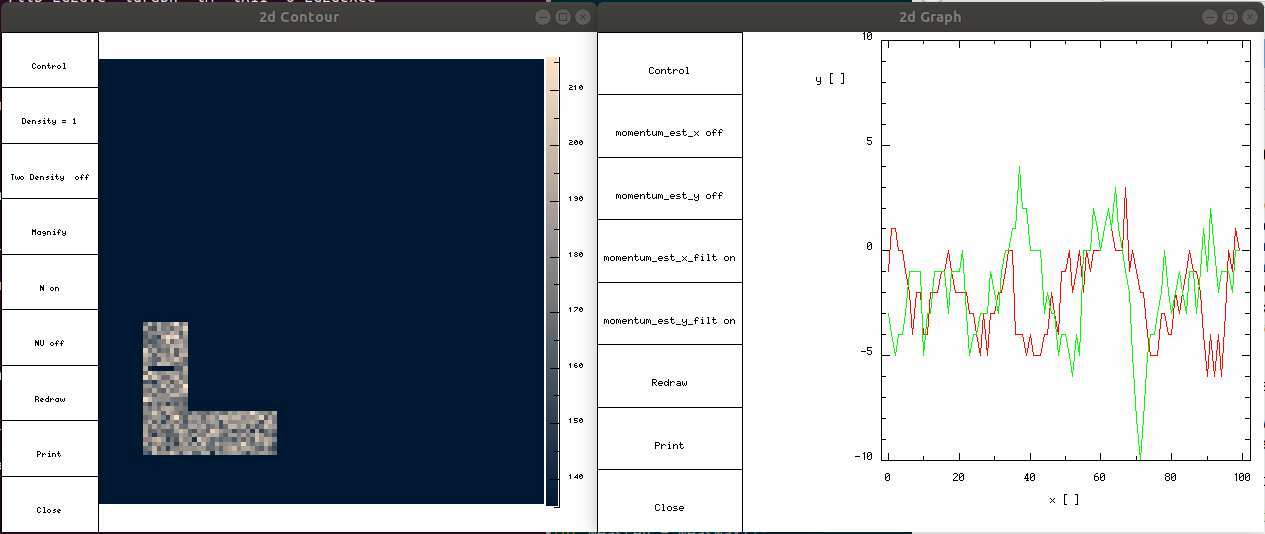
\includegraphics[scale=0.2]{p1_noleakage.png}
\caption{\label{fig} Here are several horizontal and vertical walls produced using the approach described above. The walls are containing the particles from leaving the shape. On the right hand side, there are graphs for the x and y momentum being imparted on the walls}
\end{figure}

\subsection{Approach 1}

The first approach taken to creating a moving wall was to move a wall very slowly with its velocity being much less than 1. The wall will move either dependently based on the momentum imparted on the wall due to particle collisions, or a set velocity will be given to wall.
 $$\frac{\sum_{n=1}^{nmax} -2*\textrm{net particles reflected}}{\textrm{wall mass}} = \textrm{wall velocity}$$
\vspace{5mm}

Code for calculating the wall momentum and resulting velocity
\begin{minted}{c}
    //summing all momemtums
    dynamic_wall_momentum_x += -2*vx*(n[x][y][8-v]-tmp);
    dynamic_wall_momentum_y += -2*vy*(n[x][y][8-v]-tmp);

	if(dynamic_wall_control_on == 0){
    		dynamic_wall_vx = dynamic_wall_momentum_x/wall_mass;
    		dynamic_wall_vy = dynamic_wall_momentum_y/wall_mass;
	}
\end{minted}
\vspace{5mm}

As the wall moves, it would "pass over" particles due to rest particles in the $n[x][y][0]$ state. To compensate for this, a random number of particles would be added to either side of the wall depending on the wall's velocity and the density of the particles surrounding the wall. For simplicity, a flat distribution was used ranging from 0 to the smaller density of particles on either side of the wall. This is necessary to prevent negative densities. This number of particles is refereed to as "flow".

$$
\textrm{Expected value of flow}$$\\
$$<flow> = \textrm{particle density * wall velocity}$$\\
$$0 < flow < \textrm{min particle density}$$\\




Code for calculating flow
\begin{minted}{c}
  int tmp_0 = n[(((vx+x)%XDIM)+XDIM)%XDIM][((y+vy)%YDIM+YDIM)%YDIM][8-v];
    int tmp = n[(((vx+x)%XDIM)+XDIM)%XDIM][((y+vy)%YDIM+YDIM)%YDIM][v];
	//find the smaller value to be the max for the random function to 
	//avoid having negative densisties
    //determining values for forward and backward particle flow
	int max_random = 1;
	if(tmp > tmp_0){
		max_random = tmp_0;
		}
	else{
		max_random = tmp;
		}
	if(max_random > 0){
		flow = (rand()%max_random)*dynamic_wall_vx;
		}
	else{
		flow = 0;
		}
\end{minted}
\vspace{5mm}
The following wall momentum is then:
\begin{minted}{c}
    dynamic_wall_momentum_x += -2*vx*(n[x][y][8-v]-tmp+flow);
    dynamic_wall_momentum_y += -2*vy*(n[x][y][8-v]-tmp);
    \end{minted}
\vspace{5mm}


\vspace{5mm}
Adding the flow to the lattice sites to produce a moving wall
\begin{minted}{c}
    //swapping the particles trying to enter and leave to have the effect of a wall
    n[(((vx+x)%XDIM)+XDIM)%XDIM][((y+vy)%YDIM+YDIM)%YDIM][v] = n[(((x)%XDIM)+XDIM)%XDIM][((y)%YDIM+YDIM)%YDIM][8-v] - flow;
    n[(((x)%XDIM)+XDIM)%XDIM][((y)%YDIM+YDIM)%YDIM][8-v] = tmp + flow;		
    \end{minted}
\vspace{5mm}

\subsection{Results}

Initial results were promising, but this approach did not factor in the number of particles at rest position, so there was significant particle leakage.

\begin{figure}[H]
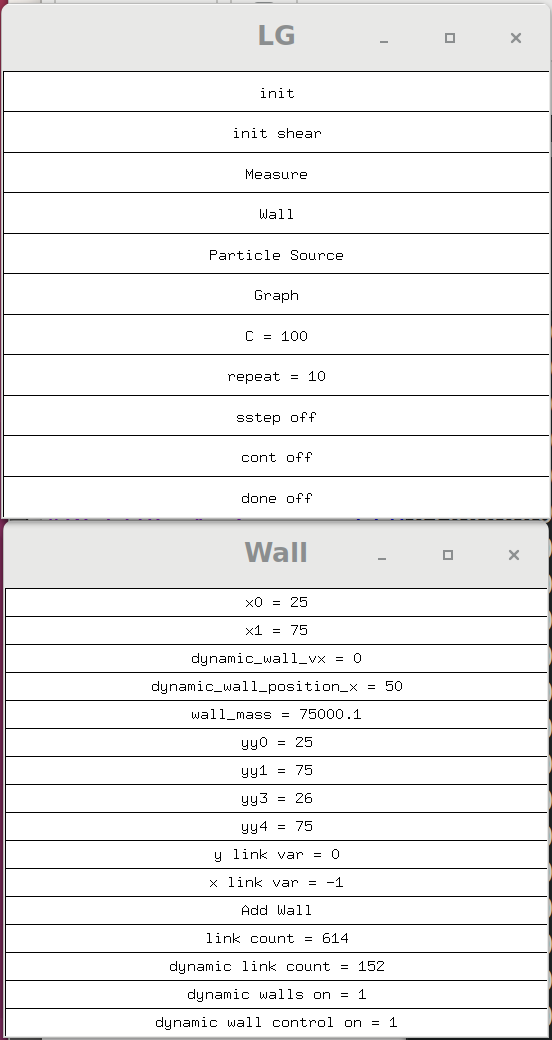
\includegraphics[scale=0.35]{A1_p0.png}
\caption{\label{fig} Settings for the simulation}
\end{figure}

\begin{figure}[H]
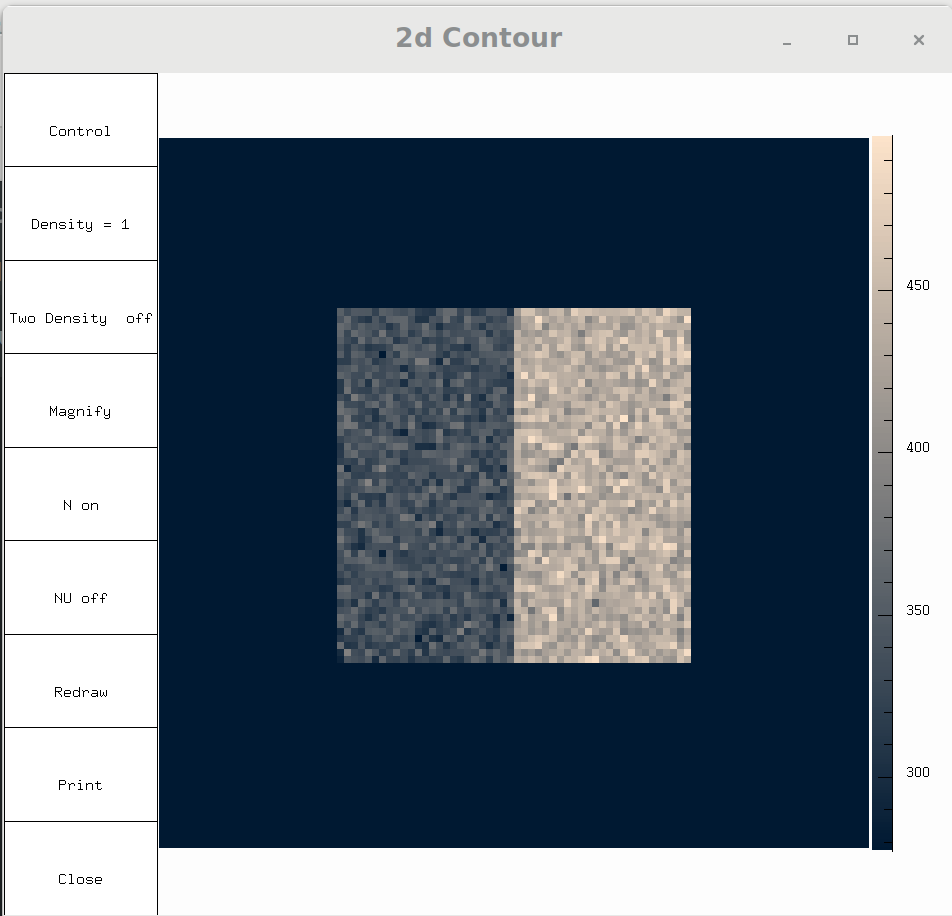
\includegraphics[scale=0.35]{A1p1.png}
\caption{\label{fig}  A box produced with static walls with one vertical dynamic wall in the center. The density on the right is 15*9 and the density on the right is 10*9. The wall is being held at position 50}
\end{figure}

\begin{figure}[H]
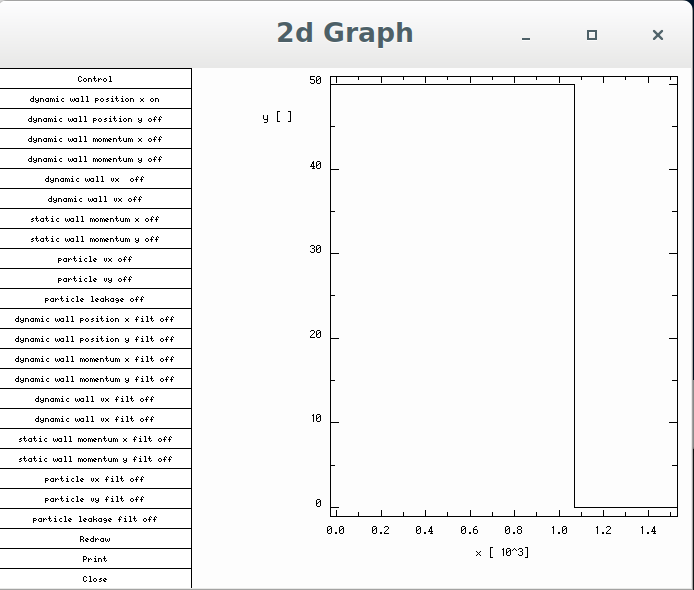
\includegraphics[scale=0.35]{A1p2.png}
\caption{\label{fig} Graph of the dynamic wall x position}
\end{figure}

\begin{figure}[H]
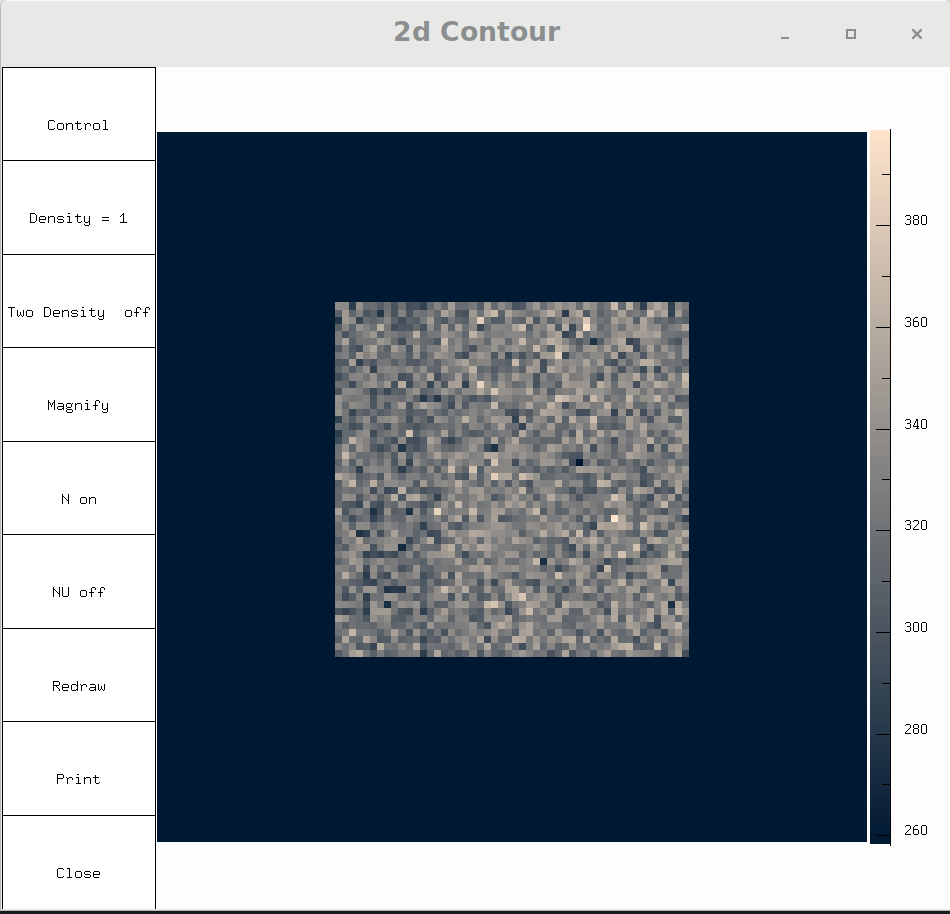
\includegraphics[scale=0.35]{A1p3.png}
\caption{\label{fig} The force keeping the dynamic wall is removed and the wall moved towards equilibrium, but it passes the theoretical equilibrium point: 45. This error is due to leakage from rest particles}
\end{figure}

\begin{figure}[H]
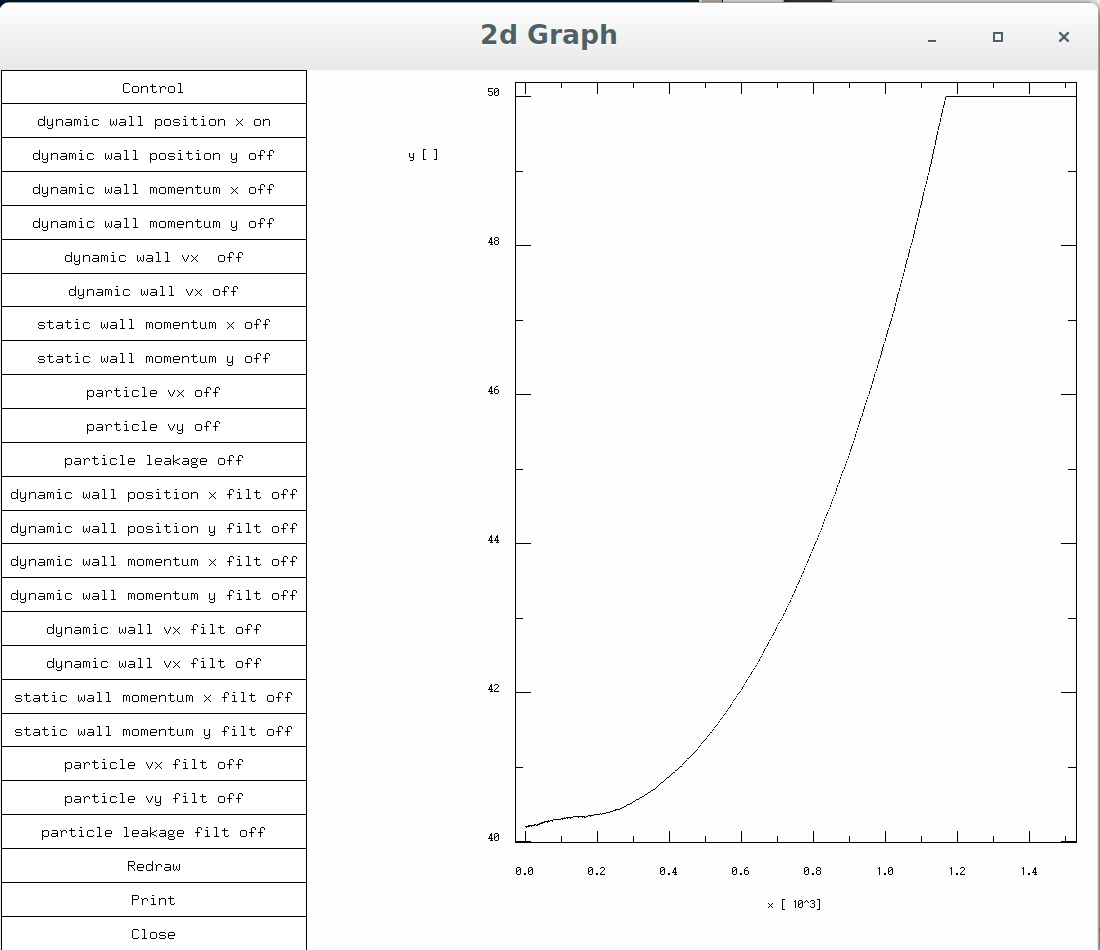
\includegraphics[scale=0.35]{A1p4.png}
\caption{\label{fig} Graph of the walls x position as it moved towards equilibrium overt time}
\end{figure}

\begin{figure}[H]
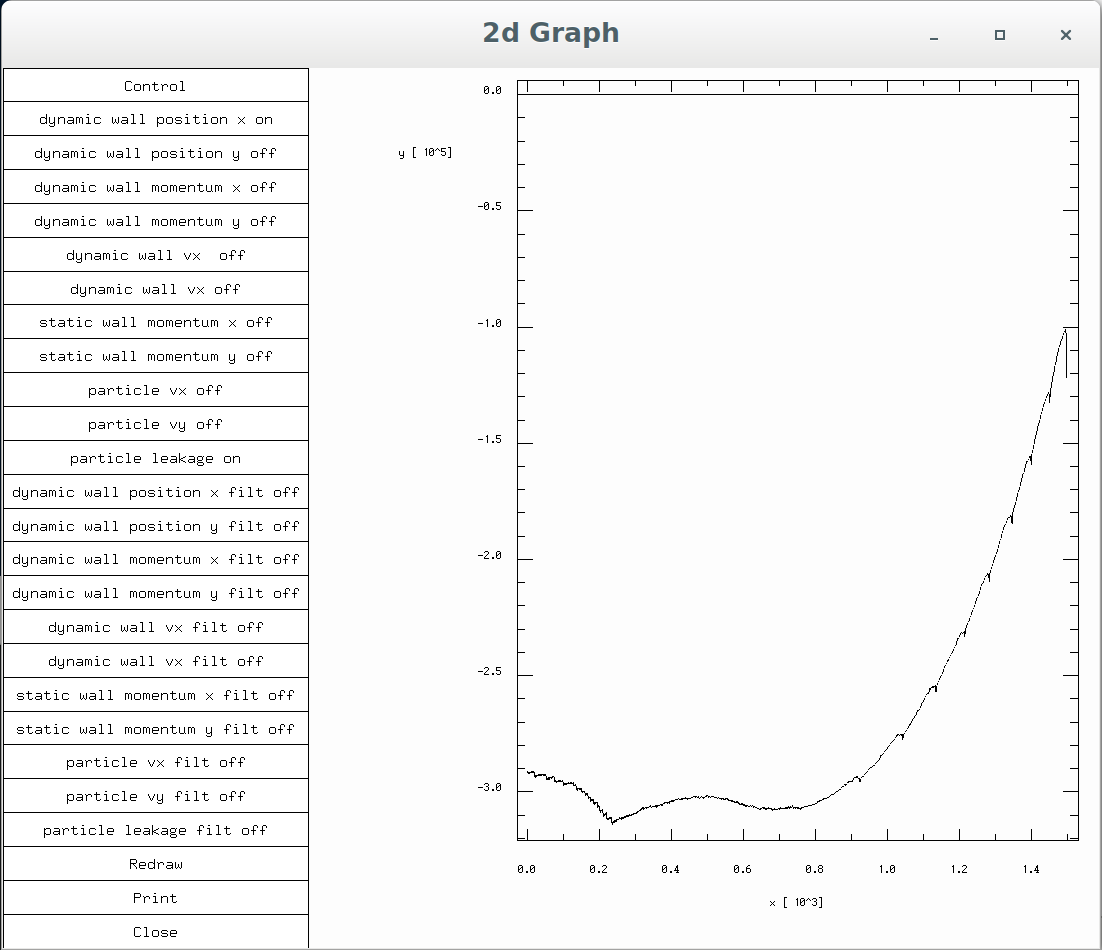
\includegraphics[scale=0.35]{A1p5.png}
\caption{\label{fig} The particles leaking through the dynamic wall as the wall moved. Note how the leakage is proportional to the walls velocity.}
\end{figure}

\subsection{Approach 2}
Approach 2 is very similar to the first approach, but the primary focus was to ensure that all the particles would be removed from the lattice site by the time the wall would exit to the next lattice site. The wall has a real number for its position whereas the lattice grid is integer, so the wall will be transitioning between lattice sites. In more detail, the probability that $$ pr * \textrm{particle density}$$ number of particles will be moved is $$pr = \frac{\textrm{Wall Vx}}{1-(\textrm{real(Wall x) - int(Wall x)})}$$. As the wall becomes closer and closer to changing lattice sites, the probability that all the particles will be moved to the next lattice site will converge to one. This is only for a case where a wall is moving to the right. This can be reproduced for a left moving wall, but was not in this program for simplicity.

\vspace{5mm}
Code added for determining the flow of particles as the wall moves.
\begin{minted}{c}
int tmp = n[x_v_b][y_v_b][v];
int iwp = dynamic_wall_position_x;//integer wall position
int flow = 0;//particles to be moved
		
double pr = dynamic_wall_vx/(1-(dynamic_wall_position_x - iwp));
//probability that p*pr particles will be moved
		if(rand()%1000 <= 1000*pr){
			flow = pr*n[x_b][y_b][v];
			n[x_b+1][y_b][v] +=flow;
			n[x_b][y_b][v] -=flow;
		}
 \end{minted}
\vspace{5mm}

\subsection{Results}

This approach had a similar amount of leaking particles as the first approach. 

\begin{figure}[H]
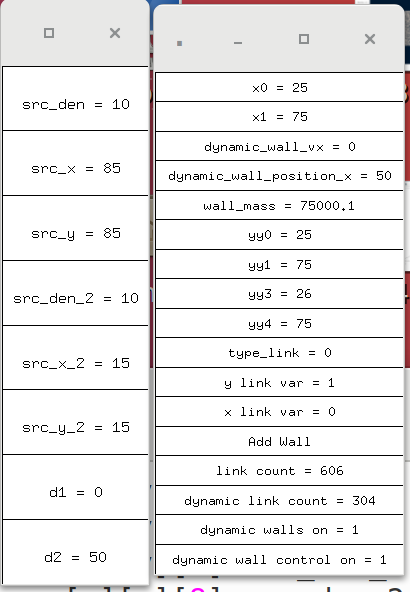
\includegraphics[scale=0.35]{A11p0.png}
\caption{\label{fig} Settings for the simulation}
\end{figure}


\begin{figure}[H]
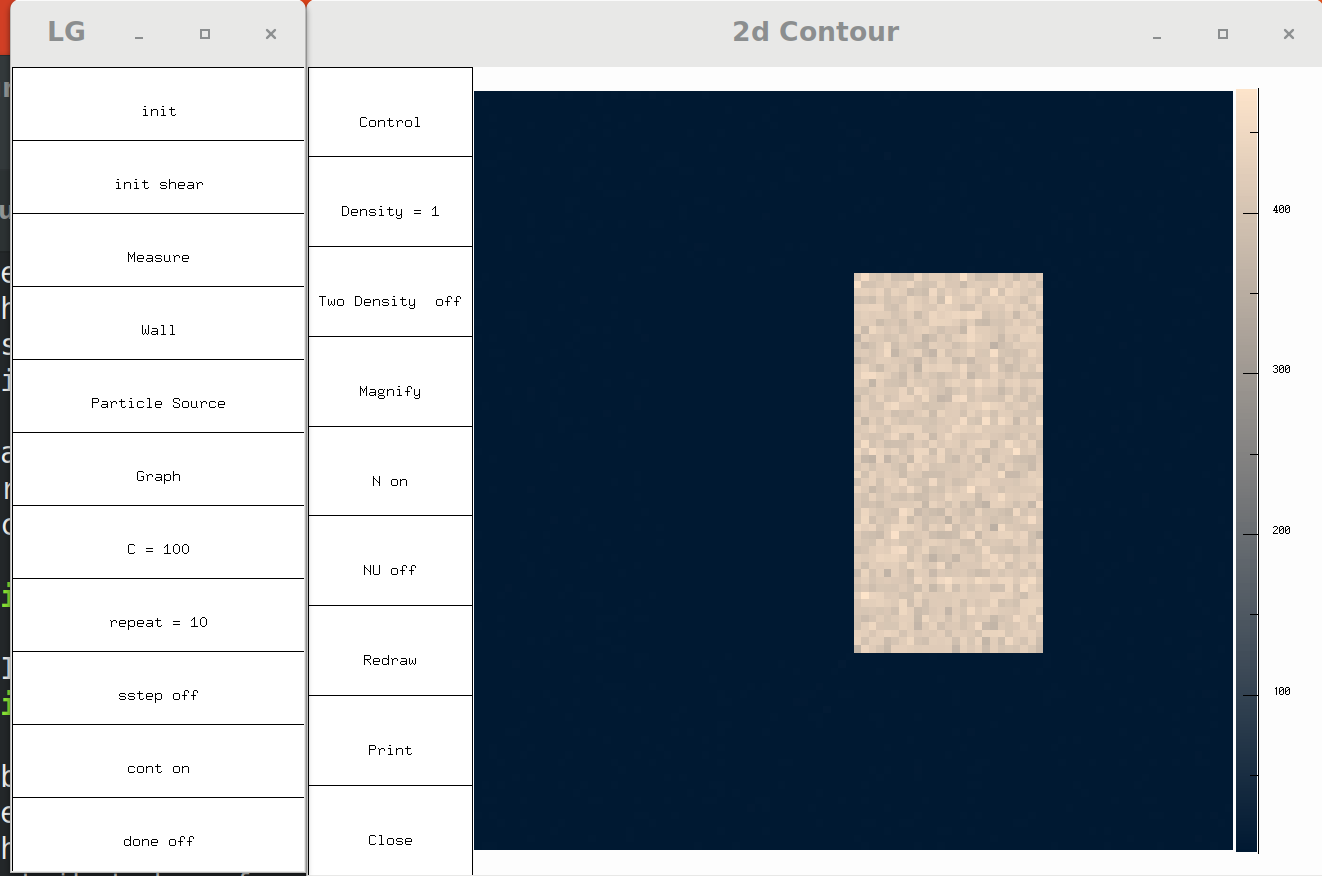
\includegraphics[scale=0.35]{A11p2.png}
\caption{\label{fig} A box produced with static walls with one vertical dynamic wall in the center. The density on the right is 50*9 and the density on the right is 0. The wall is being held at position 50. This experiment is being done to test if the wall will leak any particles. }
\end{figure}


\begin{figure}[H]
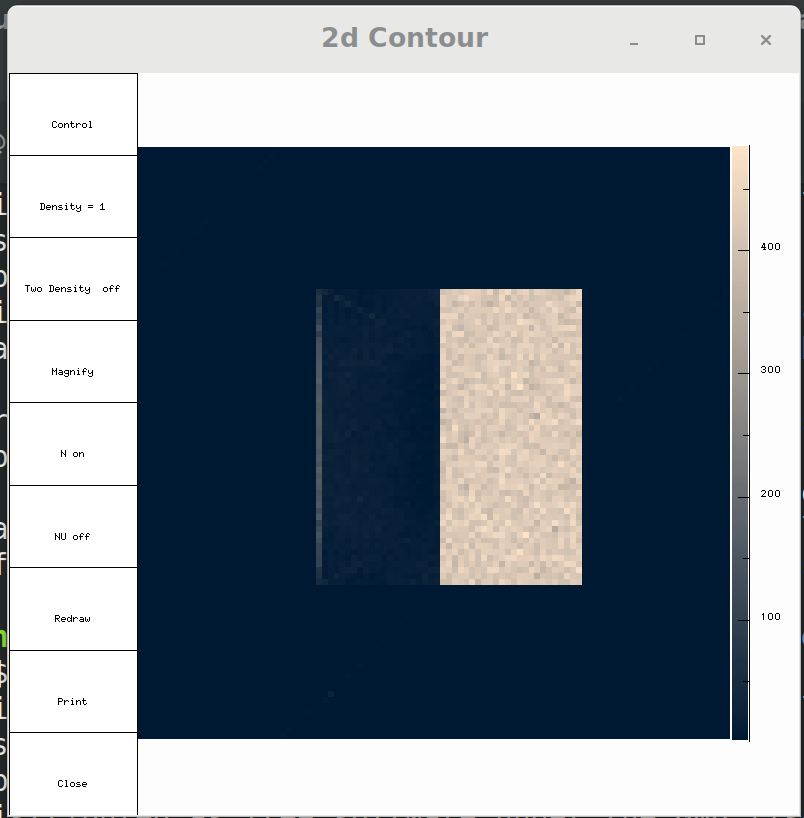
\includegraphics[scale=0.35]{A11p5.png}
\caption{\label{fig} The wall begins to move with velocity of 0.02 in the positive x direction. Notice how a notable wave of particles are being leaked when the wall changes lattice sites.}
\end{figure}


\begin{figure}[H]
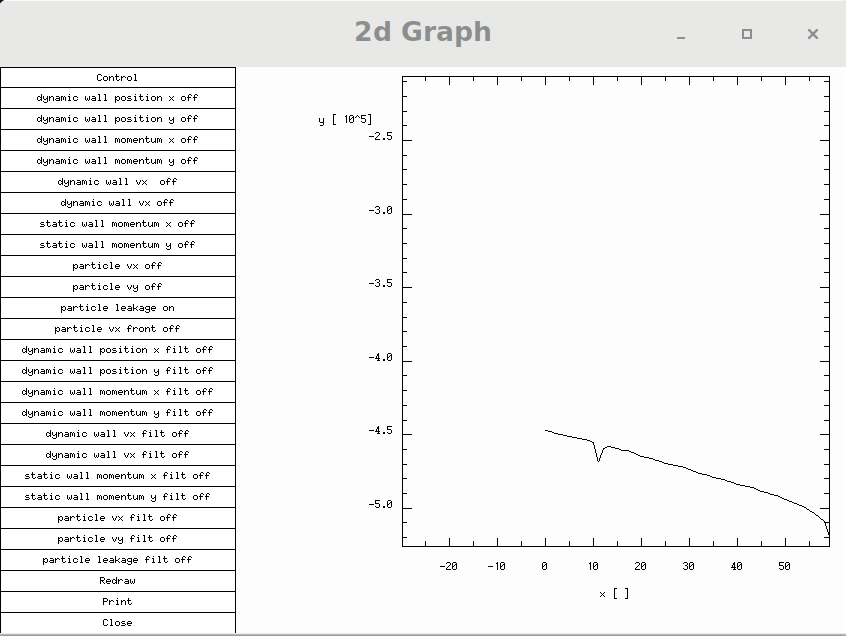
\includegraphics[scale=0.35]{A11p3.png}
\caption{\label{fig} Graph of the particles being leaked by the wall over time}
\end{figure}

\begin{figure}[H]
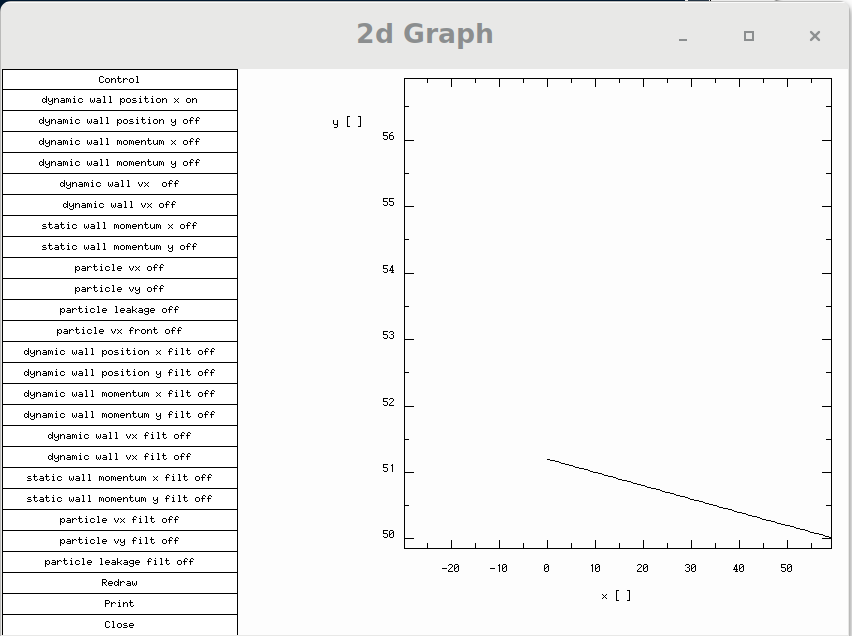
\includegraphics[scale=0.35]{A11p4.png}
\caption{\label{fig} Graph of the walls x position as it moved towards equilibrium overt time}
\end{figure}


\subsection{Approach 3}

This approach tried to simplify the program by restricting the motions of the wall, then in this specific case, the walls dynamics can be tested and verified if possible. Rest particles are still known to be causing issues, so to remove them, the walls will move into a region where there are no particles. This simulation will apply a force to particles confined by 2 walls with periodic boundary conditions allowing particles to flow from one end of the tube to the other. The walls will be static to begin with and dynamic later. The force will be applied by moving a random amount of particles from the lattice velocity states of [2 5 8] to [0 3 6]. To validate the dynamics of the simulation, the mean particle velocity with respect to the cross section of the tube will be measured in the simulation and compared to a theoretical value derived from the Navier Stokes equation for fluid dynamics.

\begin{equation}
\frac{\partial \rho}{\partial t} + \frac{\partial(\rho u_{i})}{\partial x_{i}} = \nabla(\rho) + \upsilon *\nabla(\nabla(U)+(\nabla(U)T))
\end{equation}

The partial for $\rho$ and $\rho u_{i}$ can be set to zero.
This gives us:

\begin{equation}
0 = \nabla(\rho) + \upsilon *\nabla(\nabla(U)+(\nabla(U)T))
\end{equation}


$$ \nabla(\rho) = F$$ 

\begin{equation}
0 = F + \upsilon *\nabla(\nabla(U_x))
\end{equation}

Solving the differential equation for $$U_x$$ (mean velocity) above gives us:

\begin{equation}
U_x =\frac{F}{2*\upsilon}*(x(x-L)) \textrm{Where L is the length of the tube in Lattice sites.}
\end{equation}

For C (Particle Collisions) high enough in the integer lattice gas code $$\upsilon = \frac{1}{6}$$.

\begin{equation}
U_x =\frac{F*6}{2}*(x(x-L)) \textrm{Where L is the length of the tube in Lattice sites.}
\end{equation}

The expected number of particles being moved by a set force is related to the equation below.  
\begin{equation}
<\textrm{particles moved}> = force*\rho
\end{equation}


\vspace{5mm}
Code for applying a force to the particles. The variable "particle flip w" is the force applied.
\begin{minted}{c}
void moveParticles(){
for(int x = 0;x<xdim;x++){
	for(int y = 0;y<ydim;y++){
		int flip_parts = particle_flip_w*((double)rand()/RAND_MAX)*n[x][y][5];
		n[x][y][3] += flip_parts;//n[x][y][3] + flip_parts;
		n[x][y][5] -= flip_parts;//n[x][y][5] - flip_parts;
		flip_parts = particle_flip_w*((double)rand()/(double)RAND_MAX)*n[x][y][8];
		n[x][y][6] += flip_parts;
		n[x][y][8] -= flip_parts;
		flip_parts = particle_flip_w*((double)rand()/(double)RAND_MAX)*n[x][y][2];
		n[x][y][0] += flip_parts;
		n[x][y][2] -= flip_parts;
		}
	}
}
 \end{minted}
\vspace{5mm}

Code for calculating the theoretical curve and measuring the mean x velocity of the particles

\vspace{5mm}
\begin{minted}{c}
void measure_function(){
	particle_vx = 0;
	particle_vy = 0;
	//int total_particles = 0;
	int total_particles = 0;
	double shift[ydim];
	for(int i = 0; i < YDIM -1;i++){
		total_particles = 0;
		measure_particle_velocity_front[i] = 0;
		for(int x0 = 0;x0<xdim;x0++){
			measure_particle_velocity_front[i] += n[x0][i][5]+n[x0][i][2]+n[x0][i][8] -
			 n[x0][i][3]-n[x0][i][0]-n[x0][i][6];			for(int v = 0;v<9;v++)
			  total_particles += n[x0][i][v];	
			}
		//find average particle velocity
		if(total_particles > 0){
			measure_particle_velocity_front[i] = (double)(measure_particle_velocity_front[i]/total_particles);//+shift[i];
			theoretical_particle_vx_front[i] = (double)(particle_flip_w*6.0/9.)*(i-25)*(i-75);

			}
		else{
			measure_particle_velocity_front[i] = 0;
			theoretical_particle_vx_front[i] = 0;
			}
		//setting zero point for ux
		if(ux_zero_flag == 0)ux_zero_point[i] += measure_particle_velocity_front[i];
		if(ux_zero_flag == 1)ux_zero_point[i] = (measure_particle_velocity_front[i] +
		 ux_zero_point[i])/2; 
		printf("zp = %f \n",ux_zero_point[i]);
			
		measure_particle_force_front[i] = (measure_particle_velocity_front[i] -
		 measure_particle_velocity_front_last[i]);	
		 	measure_particle_velocity_front_last[i] = measure_particle_force_front[i];
		
		}
	}

 \end{minted}
\vspace{5mm}


\subsection{Results}

There is a very large difference in the two mean velocity in the x directions, but the measured mean x velocity does show a parabolic profile like the theory suggests.

\begin{figure}[H]
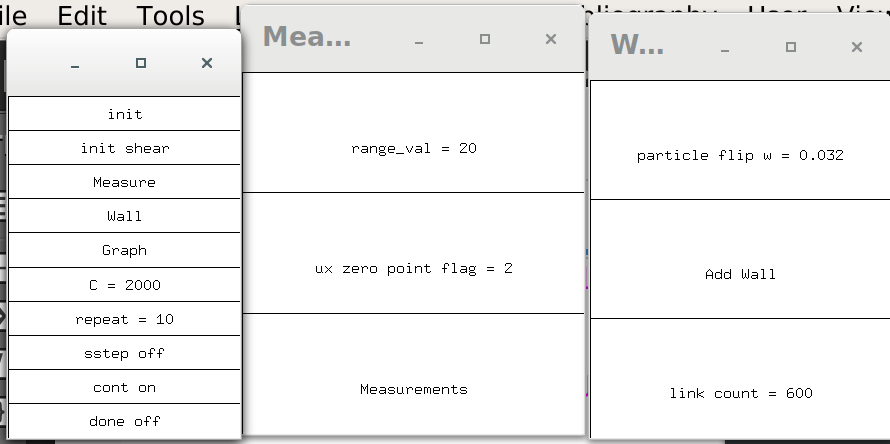
\includegraphics[scale=0.35]{A2p1.png}
\caption{\label{fig} Simulation settings}
\end{figure}

\begin{figure}[H]
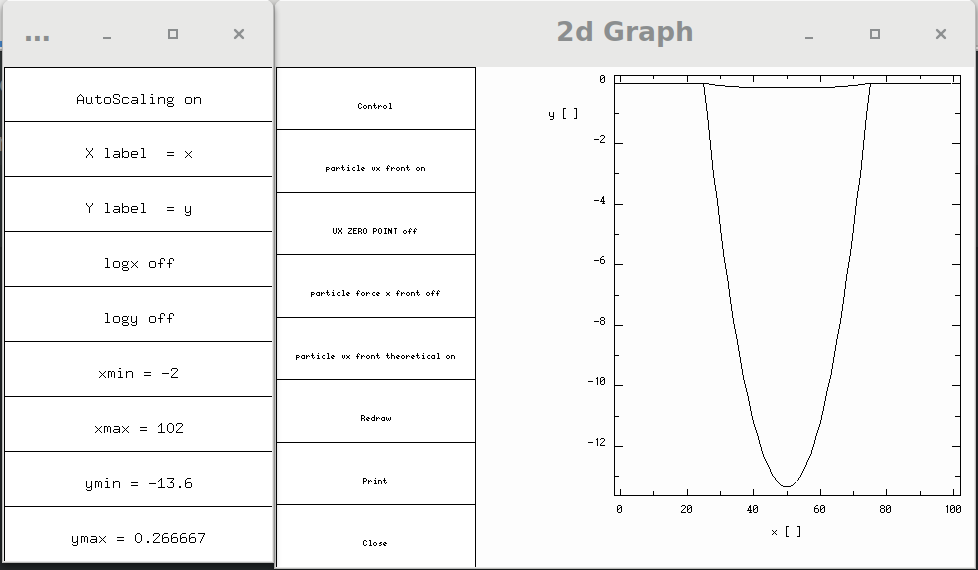
\includegraphics[scale=0.35]{A3p0.png}
\caption{\label{fig} Theoretical and measured mean particle x velocity}
\end{figure}

\begin{figure}[H]
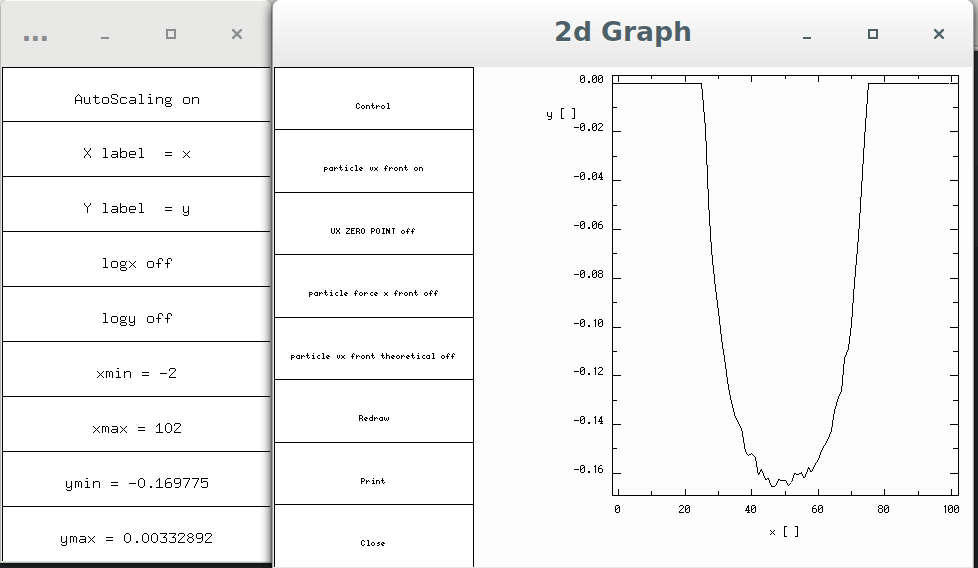
\includegraphics[scale=0.35]{A2p3.png}
\caption{\label{fig} Measured mean particle velocity x}
\end{figure}


\section{Research Group}
David Jedynak is the only undergrad working on this project.
\section{Completed Milestones}
\begin{itemize}
  \item Simulate with stationary wall and particles initially moving uniformly perpendicular to the wall. Observe how the wall influences the particles' average velocity.
 
  \item Develop code to simulate a moving wall(independent of particle collisions). Simulate with initially stationary particles. Observe how the wall influences particles average velocity. Compare results to item 1 on this list. They should have a similar result because both particles and wall are both moving with the same velocity relative to each other.
\begin{figure}

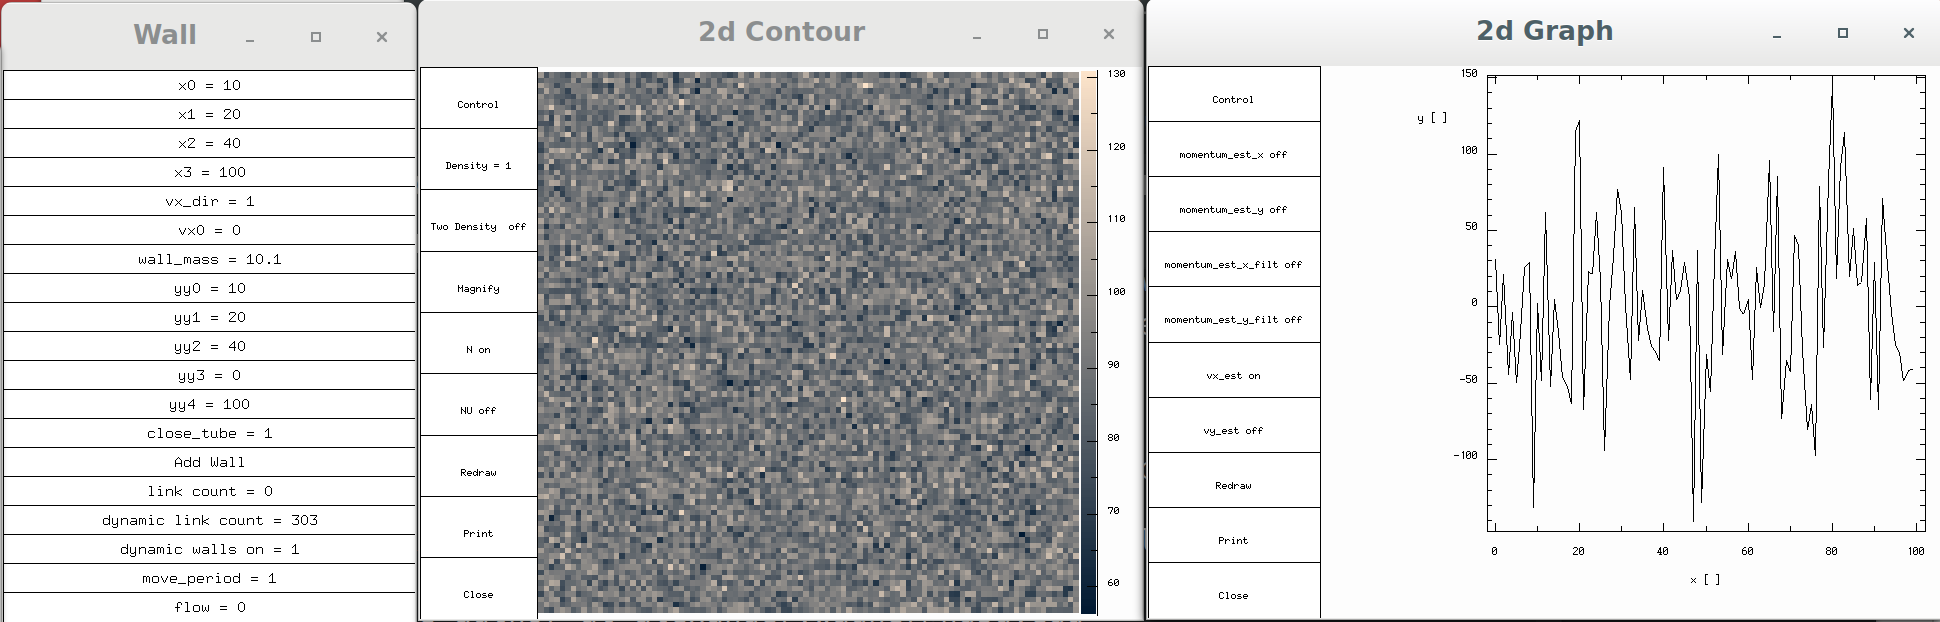
\includegraphics[scale=0.2]{ms1p0.png}
\caption{\label{fig} The 2d graph on the right hand side is the horizontal particle velocity. The contour plot is the Integer Lattice Gas Simulation with an independent moving wall. This is the simulation with the wall velocity being zero.}
\end{figure} 

\begin{figure}

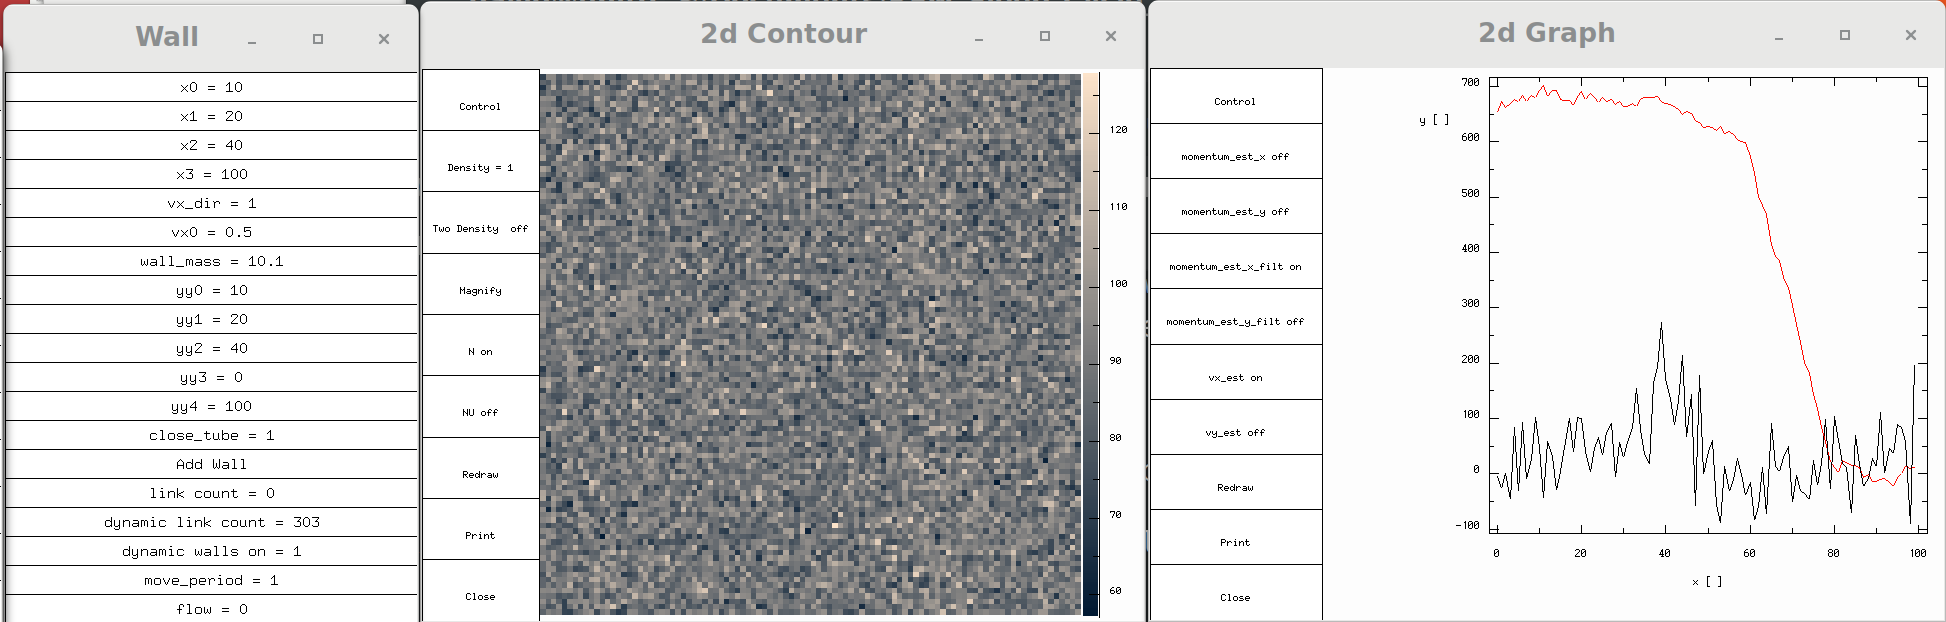
\includegraphics[scale=0.2]{ms1p1.png}
\caption{\label{fig} Several iterations later: the 2d graph on the right hand side is the horizontal particle velocity. The contour plot is the Integer Lattice Gas Simulation with an independent moving wall. This is the simulation with the wall velocity being nonzero(0.5) and positive. Observe how the particle velocity(Black) and Wall momentum (Red) increases.}
\end{figure}

\begin{figure}

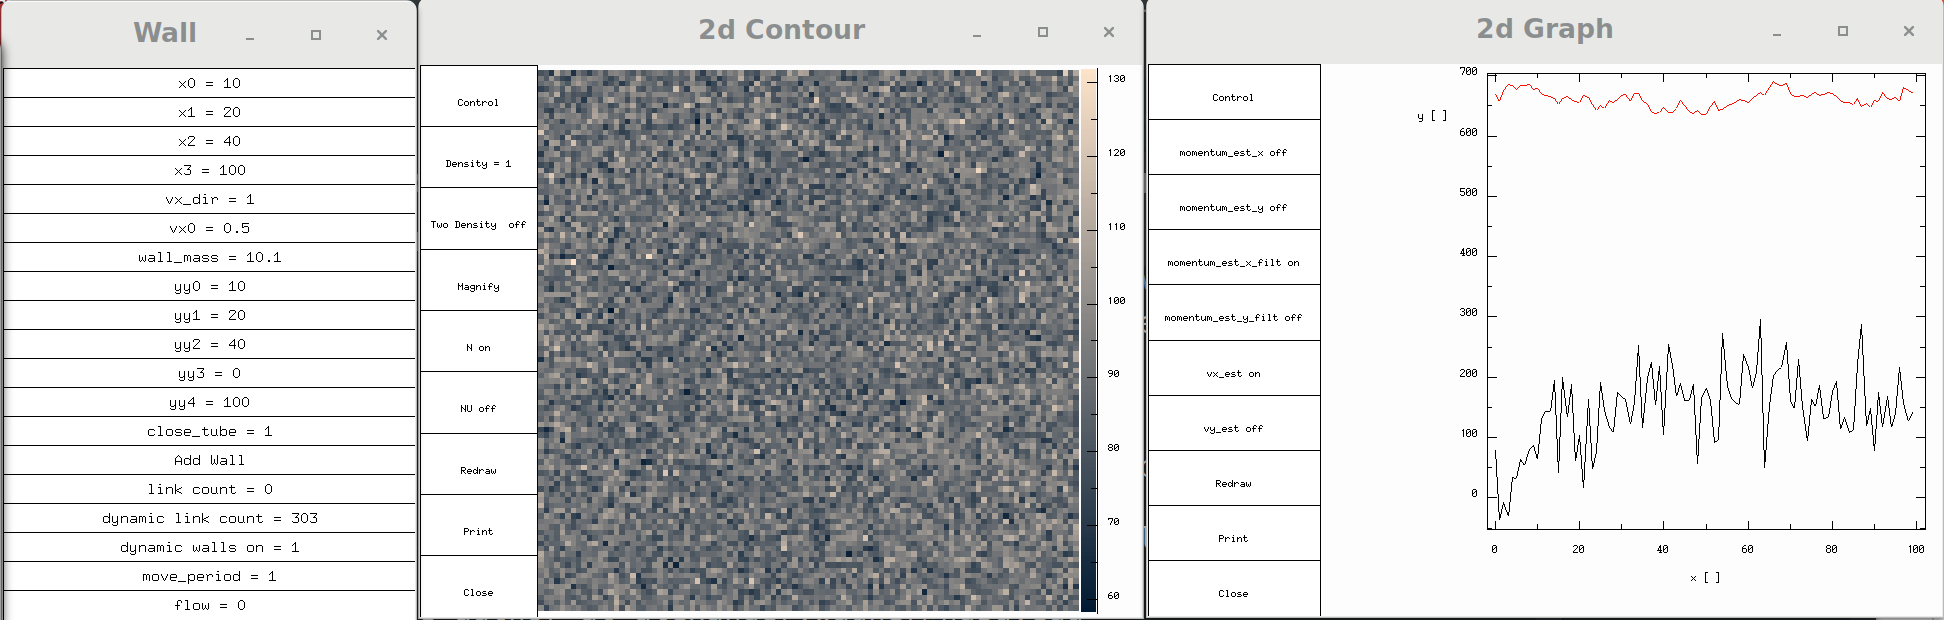
\includegraphics[scale=0.2]{ms1p2.png}
\caption{\label{fig} After running for sometime: The 2d graph on the right hand side is the horizontal particle velocity. The contour plot is the Integer Lattice Gas Simulation with an independent moving wall. This is the simulation with the wall velocity being nonzero(0.5) and positive. The total wall momentum levels off and the particle velocity levels off as well.}
\end{figure}    
 \item Develop code to make wall momentum to be dependent on particle collisions. Simulate a hollow, horizontal, stationary tube with one horizontally movable, vertical wall. place gasses in each side of the vertical wall with different densities. Observe the movement of the movable wall. The wall should stop moving when both particle densities equalize.\newline
\vspace{5mm}\newline
\begin{figure}

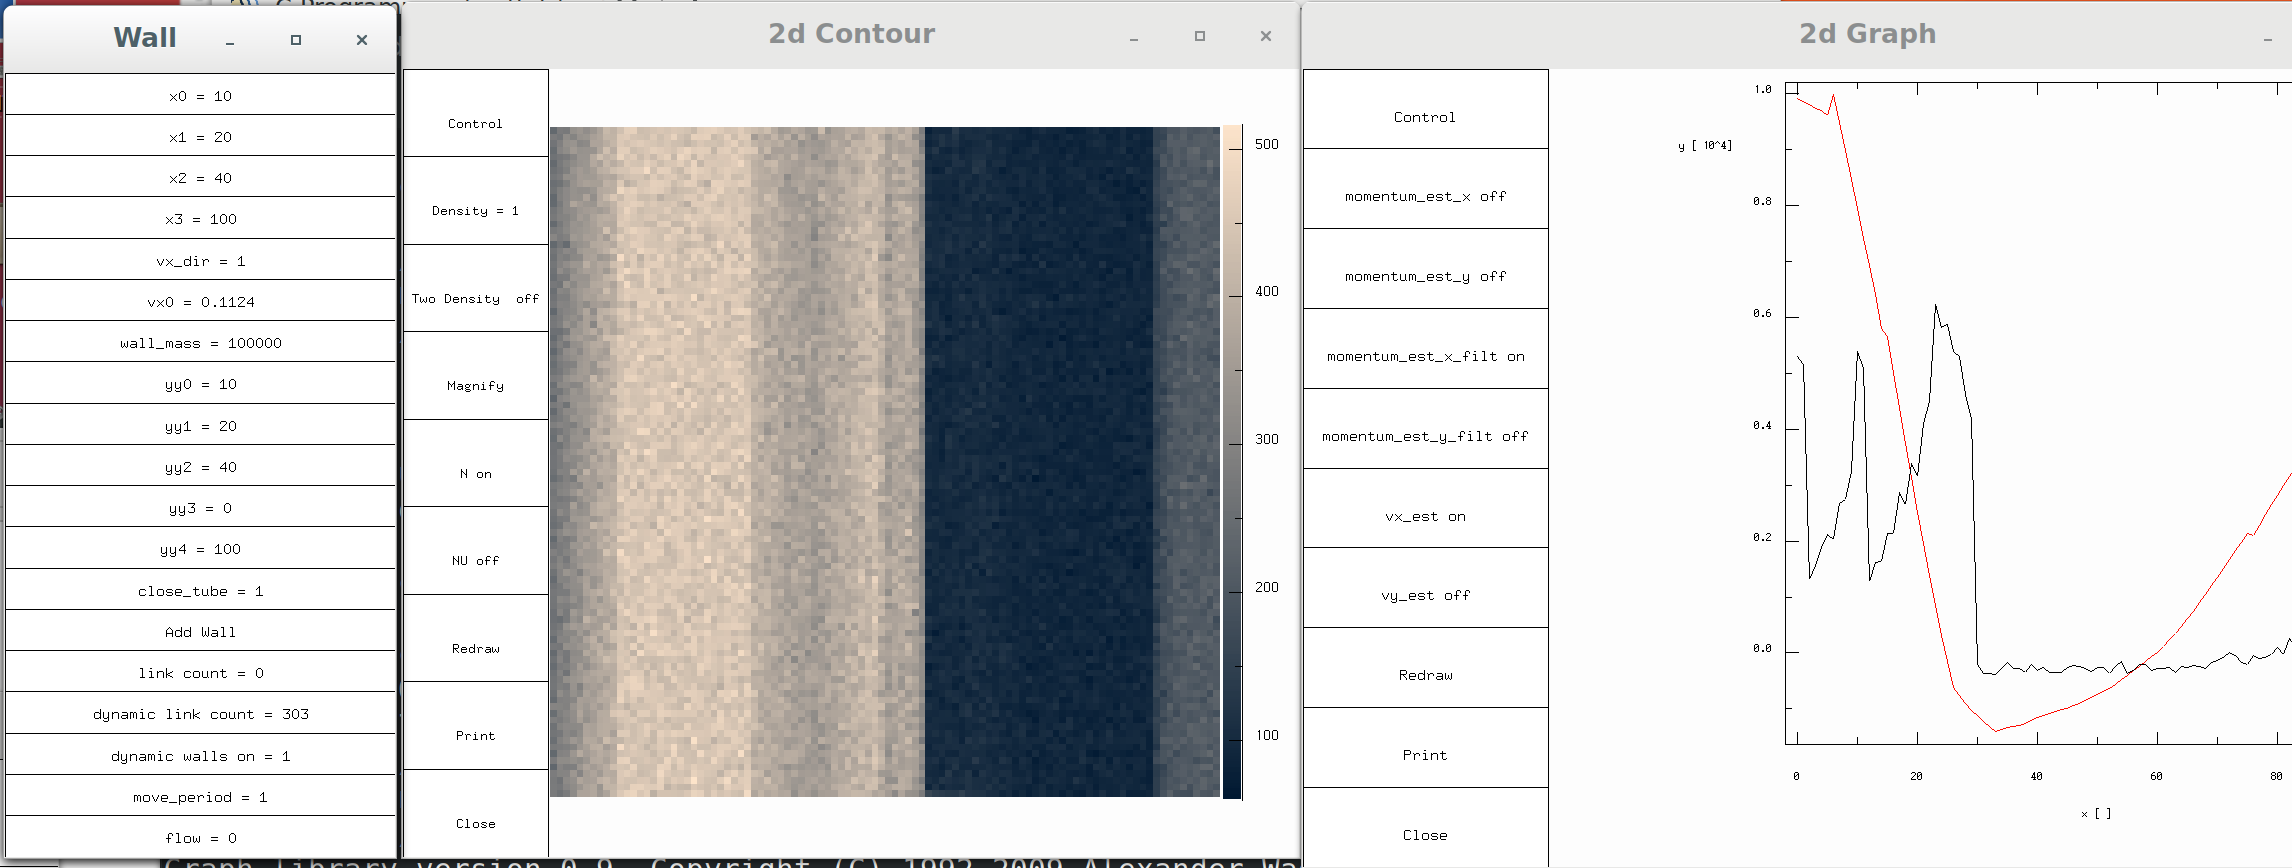
\includegraphics[scale=0.2]{ms2p0.png}
\caption{\label{fig} This is a simulation where the dynamic wall's horizontal velocity is proportional to the momentum gained by the gas particles divided by a set mass. The left hand side has particle densities of 100 from x = 0 to 40 and then densities of 20 from 60 to 100. The purpose of this experiment was to watch the wall velocity change based on particle collisions. See how the velocity (vx0 is equal to ~0.1)}
\end{figure}

\begin{figure}

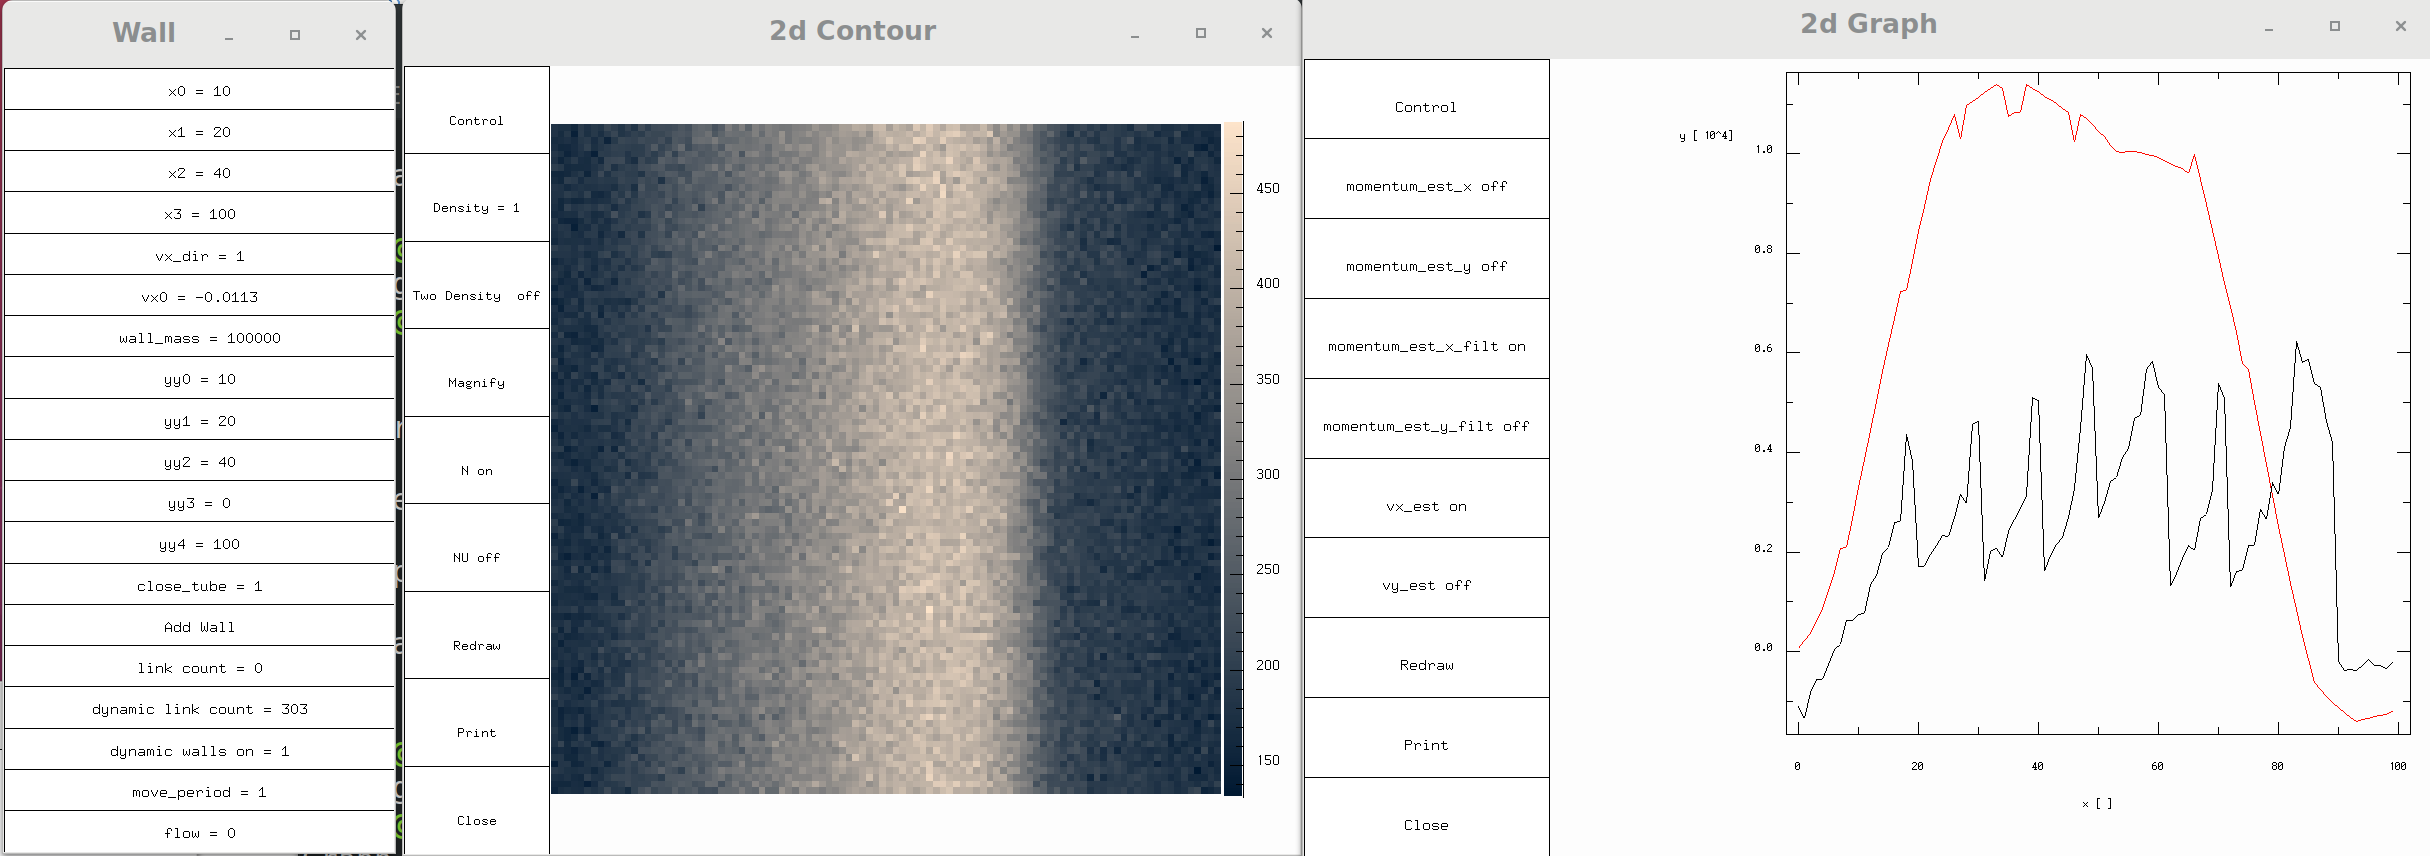
\includegraphics[scale=0.2]{ms2p1.png}
\caption{\label{fig} Several Iterations Later: the wall velocity begins to change and move towards the lower density side of the box. There seems to be some sloshing/ reflections of the particles as the velocity is now negative}
\end{figure} 

  
\end{itemize}
Some of these milestones have been revised based on information obtained while developing the code to run said simulations. 
\begin{itemize}
  
  \item Decrease the amount of particle leakage. Find a way to measure particle leakage.
  
  \item Create an architecture in the code to simplify the addition of multiple line shapes, the manipulation of their characteristics and states like mass, velocity, position. This architecture should also include the ability to create diagonal lines. (In Progress)
  
  \item develop code to allow for shapes to rotate about a center of mass or a fixed point.
  
 
Additional long term milestones could include the addition of rotating walls, hinges to connect walls, flexible walls. These features may be unrealistic with the available time, but could prove to be useful in creating more complex simulations.
\end{itemize}
\section{Timeline}
\begin{itemize}
  \item Tuesday, April 17th: Have milestone 1 and 2 completed - achieved except number 1
  \item Thursday, April 19th: Have milestone 3 started - achieved, but particles still leaking
  \item Tuesday, April 24th: Have milestone 3 completed and 4 started. (slightly behind, 3 is not entirely completed yet)
\end{itemize}
The primary objective is to have a shape/line/wall that can move and appear to push lattice gas particles like a physical wall would do in the real world. These walls in the existing program can be easily moved, but as the wall moves it will move through some particles creating a leakage. To compensate for this leakage, particles are subtracted from the lattice sites on the leaving side of the wall and the same number are added to the arriving side of the wall. The sum of the particles added or removed must be zero, must not create negative particle densities. The number of particles added is taken randomly from a flat distribution. 
\section{Research Group}
David Jedynak programs 
\section{Completed Milestones}

\section{Future Milestones}
This project will depend on the a previously developed integer lattice gas simulation: "LG2d.c". This simulation already has features similar to the ones proposed in this project such as static walls that reflect particles. Code will be added to the LG2d.c simulation to observe how particles behave when the wall is dynamic instead of static walls. 
\begin{itemize}
  \item Simulate with stationary wall and particles initially moving uniformly perpendicular to the wall. Observe how the wall influences the particles' average velocity.  
  \item Develope code to simulate a moving wall(independent of particle collisions). Simulate with initailly stationary particles. Observe how the wall influences particles average velocity. Compare results to item 1 on this list. They should have a similar result because both particles and wall are both moving with the same velocity relative to eachother.
  \item Develope code to simulate a stationary tube. Place two dynamic walls on each end of the tube with particles inside this chamber. Move walls inward. Verify particles do not leak out. Observe how the particle density changes as the chamber decreases in size. Observe the forces on the walls as the chamber size changes.
  \item Develope code to make wall momentum to be dependent on particle collisions. Simulate a hollow, hoizontal, stationary tube with one horizontally movable, vertical wall. place gasses in each side of the vertical wall with different densities. Observe the movement of the movable wall. The wall should stop moving when both particle desities equalize.\newline
\vspace{5mm}\newline
Additional long term milestones could include the addition of rotating walls, hinges to connect walls, flexible walls. These features may be unrealistic with the avaliable time, but coule prove to be useful in creating more complex simulations.
\end{itemize}
\section{Timeline}
\begin{itemize}
  \item Tuesday, April 17th: Have milestone 1 and 2 completed
  \item Thursday, April 19th: Have milestone 3 started (even if leaking particles)
  \item Tuesday, April 24th: Have milestone 3 completed and 4 started. 
  \item Thursday, April 26th: Have 4 completed.
  \item Tuesday, May 1st: Have 5 started/partially functional.
  \item Thursday, May 3rd: Have 5 completed.
  \item Tuesday, May 8th: Have results and project deliverables compiled and ready to turn in.
\end{itemize}

\end{document}

